% !TeX spellcheck = en_US
\addscenariosection{1}{Coop Scenario}{Wandering Dragons}{\images/dragon.png}

\begin{multicols*}{2}

\textbf{Author:} Niilo Salonen, Juhani Salonen

\href{https://discord.com/channels/740870068178649108/1161571991732625468/threads/1432372875658137752}{Archon Studios Discord}

\textit{The dragons of this region have grown increasingly erratic and dangerous. You and your allies have decided that the time has come to end their threat once and for all. Beware, however—some dragons have strayed from the
Dragon Utopia and now roam the land. They will strike without hesitation if they feel threatened. Your mission
is to slay all dragons in the area, both those guarding the Utopia and those wandering beyond its borders.}  % no-check-caps

\subsection*{\MakeUppercase{Scenario Length}}
This Scenario plays out over 10 Rounds.

\subsection*{\MakeUppercase{Player Setup}}
\textbf{Player Count:} 2-3 players.

\textbf{Starting Resources:} 6 \svg{gold}, 2 \svg{building_materials}, 0 \svg{valuables}

\textbf{Starting Income:} 10 \svg{gold}, 2 \svg{building_materials}, 1 \svg{valuables}

\textbf{Starting Units:}

\begin{itemize}
  \item 2 × Few of cheapest \bronze\ Units.
\end{itemize}

\textbf{Town Buildings:} \bronze\ dwelling, Citadel

\textbf{Map Tile Pool:} Each player takes 1 random Far (II-III) Map Tile.

\subsection*{\MakeUppercase{Map Setup}}
Take the following Map Tiles ($P$ stands for the number of players) and arrange them as shown in the Scenario map layout:


\begin{itemize}
  \item P × Starting (I) Map Tiles.
  \item 2P × Near (IV–V) Map Tiles.
  \item 1 × Center (VI–VII) Map Tile with Dragon Utopia.
\end{itemize}

\subsection*{\MakeUppercase{Victory Conditions}}
If all of the Units from the Dragon Utopia and the Wandering Dragons are defeated, the game ends and the players win the Scenario.

\subsection*{\MakeUppercase{Timed Events}}
\textbf{End of \nth{2} Round:}
\begin{itemize}
  \item Each player may resolve all Fields their closest starting player visited this Round. (Do not increase any income.)
\end{itemize}
\textbf{\nth{4} \& \nth{8} Round:}
\begin{itemize}
  \item Remove all Black Cubes from all Water Wheels and Windmills on the map.
\end{itemize}

\subsection*{\MakeUppercase{Additional Rules}}
Dragon Decks: With 2 players, randomly draw the following Neutral Dragon Unit Cards to two Decks (DU = Dragon Utopia, WD = Wandering Dragons):

\textbf{Easy:}
\begin{itemize}
  \item DU: 2 × \azure\
  \item WD: 2 × \golden.
\end{itemize}
\textbf{Normal:}
\begin{itemize}
  \item DU: 2 × \azure, 1 × \golden\
  \item WD: 1 × \azure, 1 × \golden.
\end{itemize}
\textbf{Hard:}
\begin{itemize}
  \item DU: 3 × \azure\
  \item WD: 1 × \azure, 2 × \golden.
\end{itemize}
\textbf{Impossible:}
\begin{itemize}
  \item DU: 3 × \azure, 1 × \golden\
  \item WD: 2 × \azure, 1 × \golden.
\end{itemize}

With 3 players, add one \golden\ Neutral Dragon to the DU Deck.

\begin{itemize}
  \item The WD starts from the Dragon Utopia and is marked with a negative Morale Token.
  \item The WD moves at the end of every Round. Roll 2 Attack Dice and add +1 to the result. On a
  \begin{itemize}
    \item +1, +2 or +3, the WD moves that amount of Fields toward the player asset (Hero, Town or Settlement) that is closest to it.
    \item 0, WD stays in place.
    \item -1, the WD moves one Field toward the DU.
  \end {itemize}
  \item If the distance is the same to two or more player assets, the WD prioritizes 1) Heroes, 2) Towns and 3)Settlements. If this does not resolve where the WD moves, a die is thrown to determine the target.

\begin{center}
  \vspace*{\fill}
  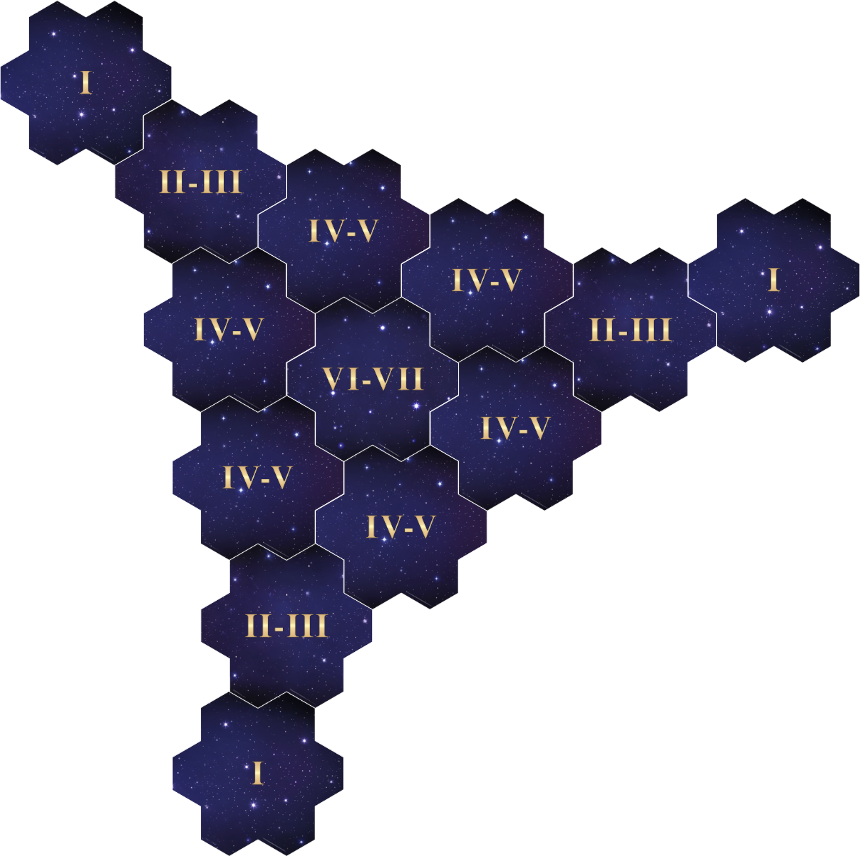
\includegraphics[width=1.2\linewidth]{\maps/wandering_dragons_3p.png}
  \captionof{figure}{\textbf{3-PLAYER SCNEARIO}}
  \vspace*{\fill}
\end{center}

\columnbreak

  \item The WD attacks if it reaches a Field with a Hero, Town or a Settlement with a Hero. In this case, the battle is fought until the end with a chance for Retreat or Surrender. If the WD reaches a Settlement without a Hero in it, the player instantly loses it.
  \item The WD may move through Blocked Fields and will end its movement on an empty Field, if possible.
  \item If the WD is defeated, the player who defeated it gains a Positive Morale token.
  \item \textbf{Obelisk:} Roll one Treasure and one Resource die and resolve both outcomes.
\end{itemize}

\vspace*{\fill}

\begin{center}
  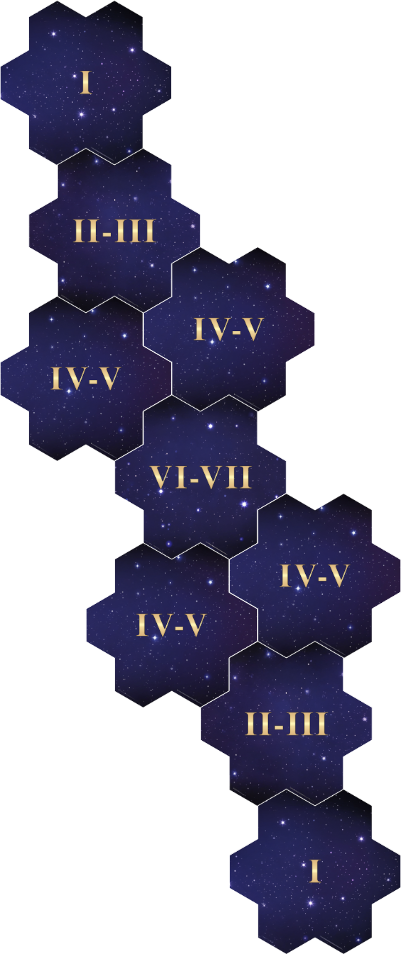
\includegraphics[width=0.6\linewidth]{\maps/wandering_dragons_2p.png}
  \captionof{figure}{\textbf{2-PLAYER SCNEARIO}}
\end{center}

\end{multicols*}
